\chapter[Documento de Arquitetura]{Documento de Arquitetura}


A finalidade do Documento de Arquitetura é definir um modelo arquitetural para ser aplicado ao desenvolvimento do sistema de anticolisões, bem como reunir todas as informações necessárias ao controle das atividades de Arquitetura, oferecendo uma visão macro dos requisitos arquiteturais e não funcionais para suportar.

\begin{enumerate}
\item \textbf{Metas e restrições da Arquitetura}

O sistema anticolisões tem por objetivo ser um sistema  que auxilia a tomada de decisões na hora da ultrapassagem . Por isso, o sistema  deverá ser seguro e sem falhas. Além disso, a arquitetura do sistema deve ser implementada de modo a permitir a evolução e manutenção do sistema. Abaixo, estão listados os requisitos que devem ser considerados para a arquitetura do sistema:

\begin{enumerate}
  \item Segurança: o sistema deve informar a distância dos carros em relação ao motorista, o sistema deve informar a possibilidade de uma ultrapassagem
  \item Disponibilidade: O sistema deverá estar disponível e ativo 24 horas por dia e 7 dias por semana.
  \item Suportabilidade: O sistema deverá funcionar em um volkswagen Gol 1.0 do ano de 2013.
\end{enumerate}

\item \textbf{Visão de Camadas}

\begin{figure}[h]
  \centering
  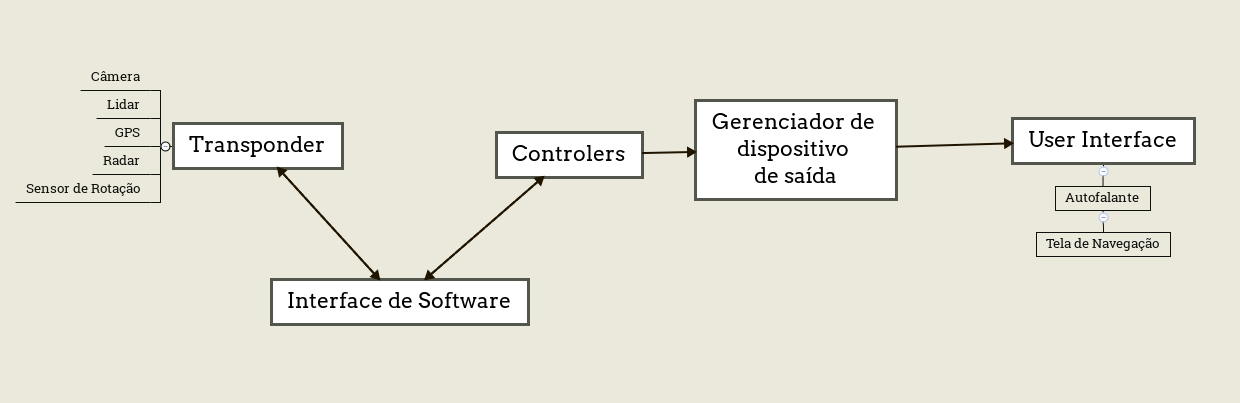
\includegraphics[width=400px, scale=1]{figuras/modelo_arquitetura}
  \caption{Modelo arquitetural do sistema}
\label{fig:modelo_arquitetura}
\end{figure}



\begin{enumerate}
  \item \textbf{Transponder:}  O transponder é responsável por receber as informações de outros dispositivos eletronicos e realizar a transmissão para o processamento do software.
  \item  \textbf{Interface de software:} Camada responsável por receber as informações que vem dos dispositivos eletronicos do sistema, e converte-los em informações que podem ser processadas pelo software
  \item \textbf{Controlers:}  Camada responsável por processar as informações que serão transmitidas dos dispositivos eletrônicos.
  \item \textbf{Gerenciador de dispositivo de saída:}  Camada responsável por fazer a conversão das informações processadas pelo sistema, para os dispositivos que utilizam recursos gráficos para o motorista.
  \item \textbf{User interface:}  Camada responsável por permitir a visualização a partir de uma interface gráfica para o motorista, lembrando que essa interface deve ser de fácil aprendizagem de uso. Devemos utilizar como referência o seguinte sistema:
\end{enumerate}

\begin{figure}[h]
  \centering
  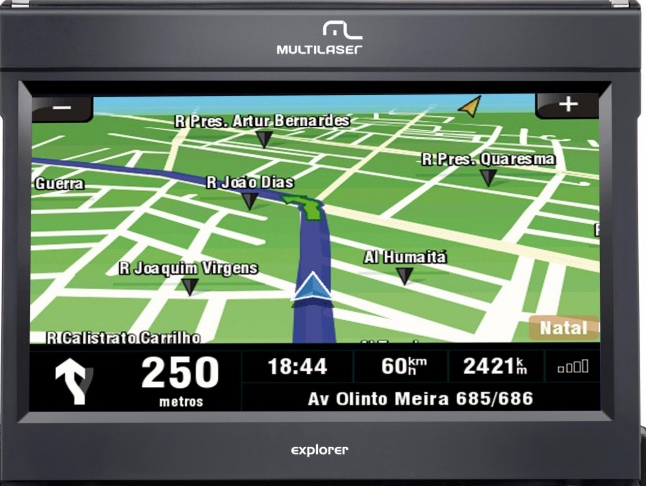
\includegraphics[width=250px, scale=1]{figuras/tela_gps}
  \caption{Modelo da tela do sistema}
\label{fig:tela_gps}
\end{figure}

\item \textbf{Visão de Implementação}
Essa seção fornece uma visão geral do modelo de implementação e da organização em termos de componentes do sistema.

\begin{enumerate}
  \item \textbf{Visão Geral}

  O diagrama de classes auxilia a visualização das classes existentes no sistema, seus atributos e seu métodos. A partir dele, também é visível o relacionamento entre as classes e também a cardinalidade entre elas. A imagem abaixo ilustra o diagrama de classe do sistema:

  \item \textbf{Diagrama de Classe }
  \begin{figure}[h]
    \centering
    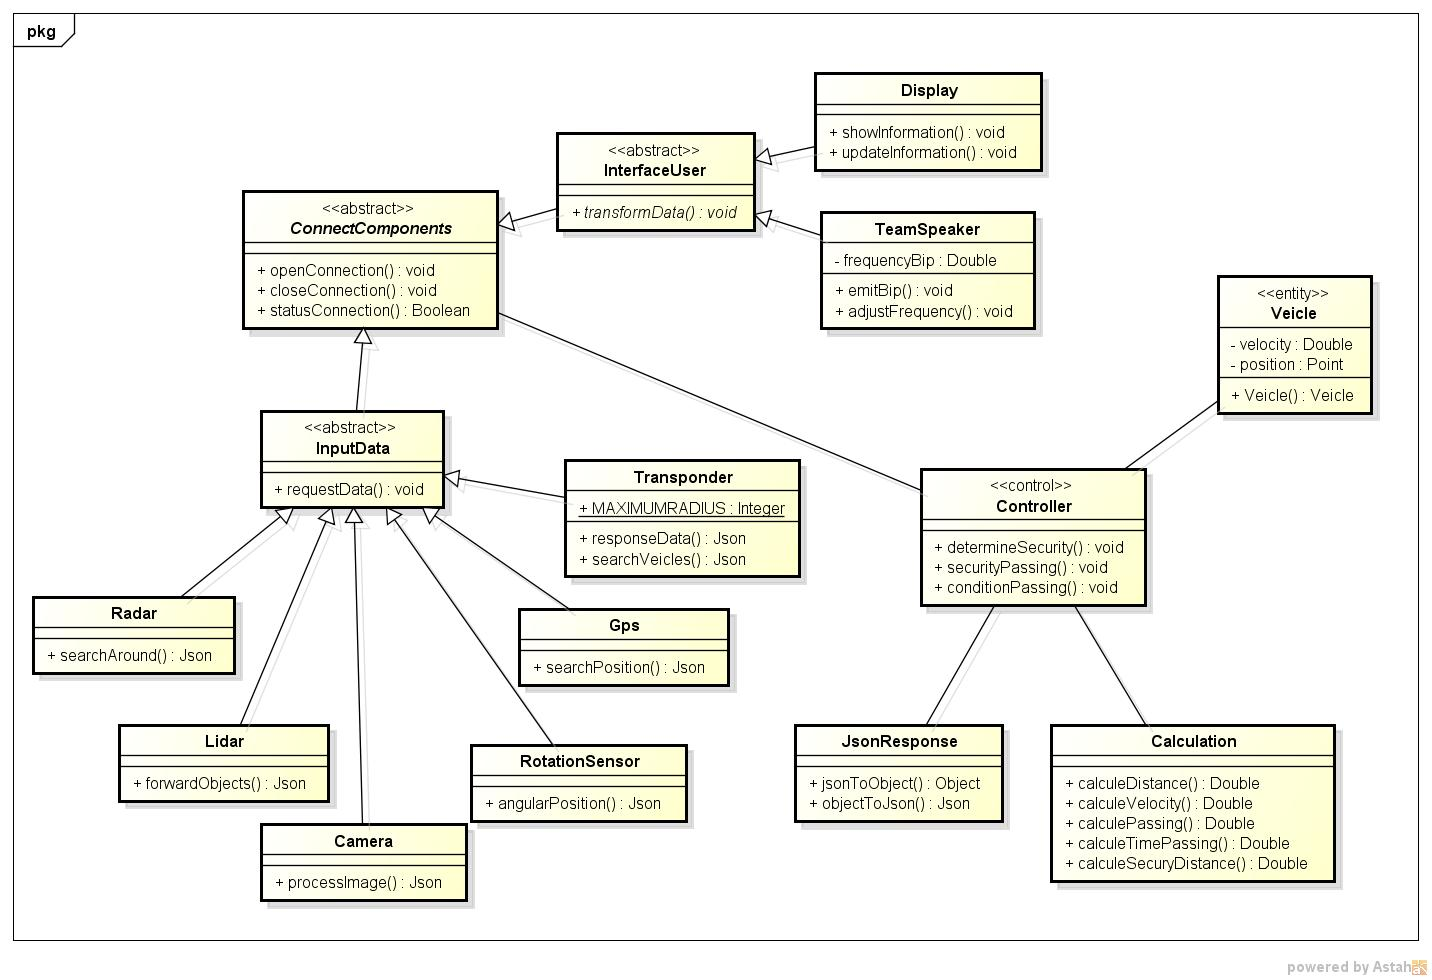
\includegraphics[width=450px, scale=1]{figuras/diagrama_classes}
    \caption{Diagrama de Classes do sistema}
  \label{fig:diagrama_classes}
  \end{figure}

\end{enumerate}
\end{enumerate}
  \begin{enumerate}
  \item Transponder:

  \item  \textbf{Transponder}: Classe que faz conexão com o transponder, para enviar e receber dados dos dispositivos de outros veículos.

\item  \textbf{Interface de software:}

ConnectComponents: Classe abstrata presente na camada de interface de software responsável por abrir ou fechar conexão com os componentes eletrônicos.

InputData: Classe abstrata para fazer a requisição ou recepção dos dados enviados pelos componentes.

Gps: Classe que realiza conexão com o gps e faz a requisição da posição caso, este não esteja mandando as informações constantemente.

RotationSensor: Classe para realizar conexão com o sensor de rotação e enviar a posição do volante quando requisitado.

Camera: Classe que conecta com o software de interface da câmera e envia as informações processadas pelo seu próprio controlador.

Lidar: Classe que conecta-se com o lidar para receber informações vindas do componente eletrônico.

Radar: Classe que conecta-se com o radar para processar as informações vindas do componente

JsonResponse: Classe que recebe as informações das classes de conexão com os dispositivos eletrônicos e transforma em objetos do software para serem usados pelas classes da camada controllers.

\item   \textbf{Controllers:}

Controller: Principal classe do sistema que irá gerenciar a comunicação com as classes que fazem comunicação com outros componentes. Processar os resultados dos cálculos realizados para indicar se favorecem a ultrapassagem com segurança.

Calculation: Classe responsável por implementar os algoritmos matemáticos otimizados para o cálculo da distância entre veículos, a velocidade ideal, o tempo necessário e a distância segura para realizar a ultrapassagem.


\item   \textbf{Gerenciador de dispositivo de saída:}

InterfaceUser: Classe abstrata que recebe as informações processadas pela camada controller e converte para dados a serem enviados para os dispositivos de comunicação com o usuário.

Display: Classe que se conecta com o display para o usuário e envia as informações a serem exibidas na tela, ou faz a atualização delas.

TeamSpeaker: Classe que conecta com o dispositivo de saída auto falante e controla a as informações sonoras a serem emitidas.




\end{enumerate}
